\section{Application: how fast do markets absorb macroeconomic news?}\label{sec:application}

\paragraph{Data.} The calendar covers January 2022--August 2026: 670 scheduled releases of
CPI, nonfarm payrolls, PPI, retail sales, the GDP advance estimate and initial jobless
claims (dated by their initial ALFRED vintage), FOMC statements and press conferences, ECB
decisions and press conferences, and Bank of Japan decisions. Surprises are standardised,
sign-split differences between the first print and a real-time expectation: the Cleveland
Fed inflation nowcast (CPI), Atlanta Fed GDPNow (GDP) and real-time statistical expectations
from earlier first prints otherwise. Prices are millisecond quotes for EUR/USD, USD/JPY,
gold and an S\&P~500 CFD, and Binance futures trades for bitcoin and ether, converted to up
and down $\delta$-crossing events ($\delta=0.25$--$3$ basis points per asset, chosen so that
the median rate is about 0.2 events per second). Windows span 30 minutes before to 60 minutes
after each release cluster, with 30 minutes of burn-in. Each window is matched with a placebo
window at the same clock times on the same weekday one to six weeks away, with no modelled
release and none of sixteen second-tier releases within three hours; placebo windows carry
their own per-type pseudo-releases, so the test is part of the likelihood. The pooled model
has \nWindows{} windows (\nNewsWindows{} release, \nPlaceboWindows{} placebo),
\nEventsScored{} million scored events and twelve dimensions, and is certified optimal to
within \gapMaxPooled{} nats per dimension.

\paragraph{Endogeneity.} The spectral radius of the branching matrix is
$\rho(G)=\rhoPooled$: roughly seven in every eight price events are echoes of earlier ones.
Fitted year by year, $\rho(G)$ declines from 2022 to 2026 (\rhoByYear), and the slowest echo
mode relaxes in about \relaxPooled{} minutes.

\paragraph{Falsification.} Nonnegative news kernels have a positive expected mass even under
the null (boundary bias), so a release-free placebo is essential. With an exposure-weighted
$\ell_1$ level chosen by held-out likelihood, \nPassPlacebo{} of the \nKinds{} release types
exceed their placebo by at least 50\% (Figure~\ref{fig:placebo}): CPI (\placeboCpi$\times$),
payrolls (\placeboNfp$\times$), PPI (\placeboPpi$\times$), the FOMC statement
(\placeboFomc$\times$) and retail sales (\placeboRetail$\times$). Jobless claims, ECB and BoJ
decisions and the press conferences have no detectable direct effect beyond their placebos.
Two earlier specifications failed this test and are reported in Appendix~\ref{app:history}.

\begin{figure}[!htbp]\centering
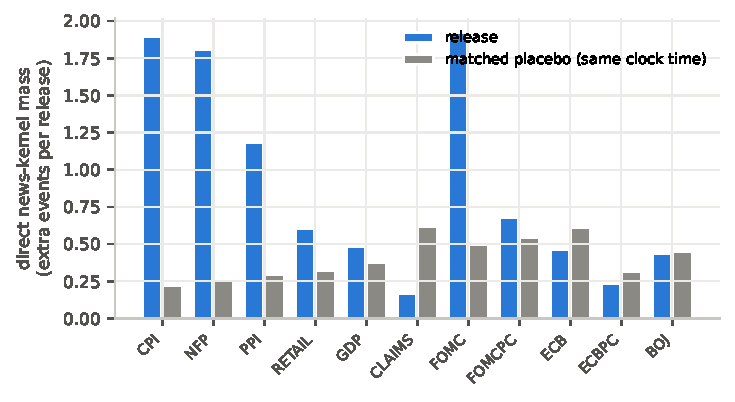
\includegraphics[width=0.72\linewidth]{figures/placebo_pooled.pdf}
\caption{Placebo test: direct news-kernel mass (expected extra events per release, all
assets) for each release type and for its matched placebo on release-free days.}\label{fig:placebo}
\end{figure}

\paragraph{Echo-corrected absorption.} For the releases that pass, the direct news kernel is
absorbed almost instantly (median $t_{50}$ of \tDirMed{}\,s), but echoes stretch the response:
half of the extra activity arrives within \tEchoLo--\tEchoHi{}\,s and ninety percent within
\tNinetyLo--\tNinetyHi{} minutes (Figure~\ref{fig:absorption}, Table~\ref{tab:absorption}).
The ``news half-life'' $\ln2/\beta$ therefore understates absorption time by one to two orders
of magnitude. Because signed surprises enter the news kernel separately by sign, the model also
gives price-discovery curves (Figure~\ref{fig:drift}, Table~\ref{tab:drift}); hotter inflation
lowers bitcoin and ether, cooler inflation lifts them.

\begin{figure}[!htbp]\centering
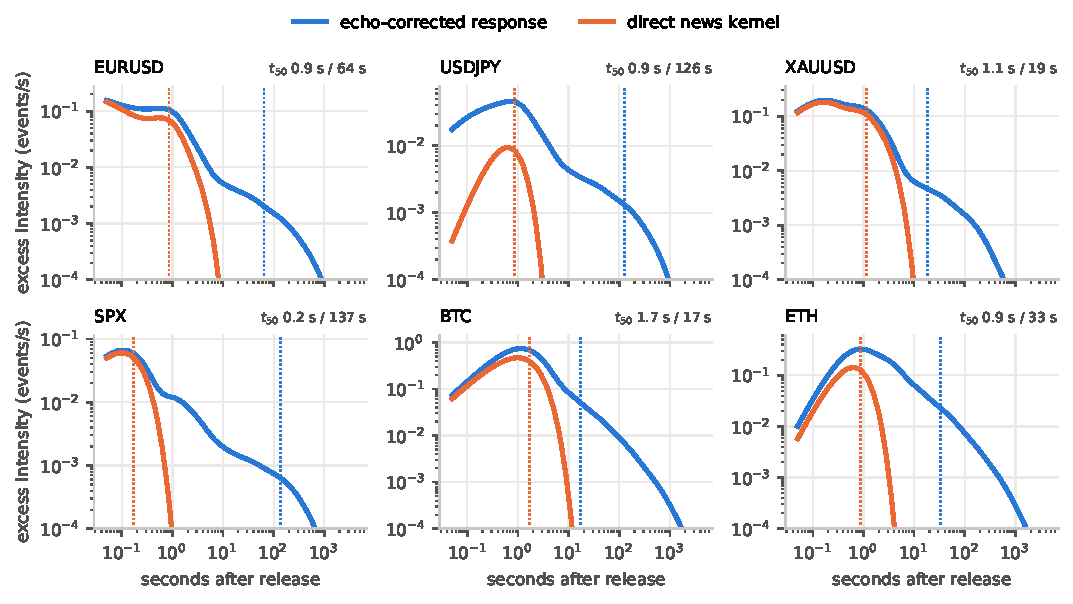
\includegraphics[width=\linewidth]{figures/absorption_CPI_pooled.pdf}
\caption{Echo-corrected response to a CPI release (blue) versus the direct news kernel
(orange), per asset; dotted lines mark $t_{50}$.}\label{fig:absorption}
\end{figure}

\begin{table}[!htbp]\centering\small
\caption{Echo-corrected absorption by release and asset: $t_{50}$ in seconds / $t_{90}$ in
minutes. $^\ast$Release types that do not exceed their placebo by 50\%.}\label{tab:absorption}
\setlength{\tabcolsep}{4pt}
\begin{tabular}{lcccccc}
\toprule
Release & EURUSD & USDJPY & Gold & S\&P 500 & BTC & ETH \\
\midrule
CPI & 64 / 9.1 & 126 / 11.0 & 19 / 4.8 & 137 / 11.0 & 17 / 6.1 & 33 / 7.8 \\
NFP & 94 / 10.1 & 109 / 10.7 & 16 / 5.2 & 80 / 8.8 & 27 / 7.5 & 24 / 7.3 \\
PPI & 120 / 10.8 & 94 / 10.3 & 40 / 6.4 & 79 / 8.6 & 23 / 7.2 & 39 / 8.7 \\
FOMC & 89 / 10.1 & 76 / 9.8 & 82 / 9.0 & 77 / 8.9 & 41 / 9.2 & 36 / 9.1 \\
Retail & 59 / 9.1 & 77 / 9.8 & 87 / 9.2 & 114 / 10.4 & 26 / 7.6 & 26 / 7.8 \\
\midrule
GDP$^\ast$ & 95 / 10.0 & 81 / 9.6 & 26 / 5.1 & 145 / 11.2 & 27 / 7.3 & 27 / 7.5 \\
FOMC press conf.$^\ast$ & 88 / 10.0 & 111 / 10.9 & 60 / 8.1 & 59 / 8.0 & 45 / 9.5 & 52 / 10.0 \\
Claims$^\ast$ & 124 / 11.0 & 56 / 9.1 & 87 / 9.3 & 81 / 9.1 & 36 / 9.0 & 40 / 9.4 \\
ECB$^\ast$ & 61 / 9.2 & 73 / 9.6 & 88 / 9.0 & 123 / 10.8 & 37 / 9.2 & 42 / 9.6 \\
ECB press conf.$^\ast$ & 137 / 11.3 & 90 / 10.2 & 38 / 6.5 & 63 / 8.2 & 25 / 7.3 & 32 / 8.0 \\
BoJ$^\ast$ & 93 / 10.2 & 80 / 9.9 & 45 / 7.3 & 73 / 8.8 & 35 / 8.5 & 37 / 8.8 \\
\bottomrule
\end{tabular}
\end{table}

\begin{figure}[!htbp]\centering
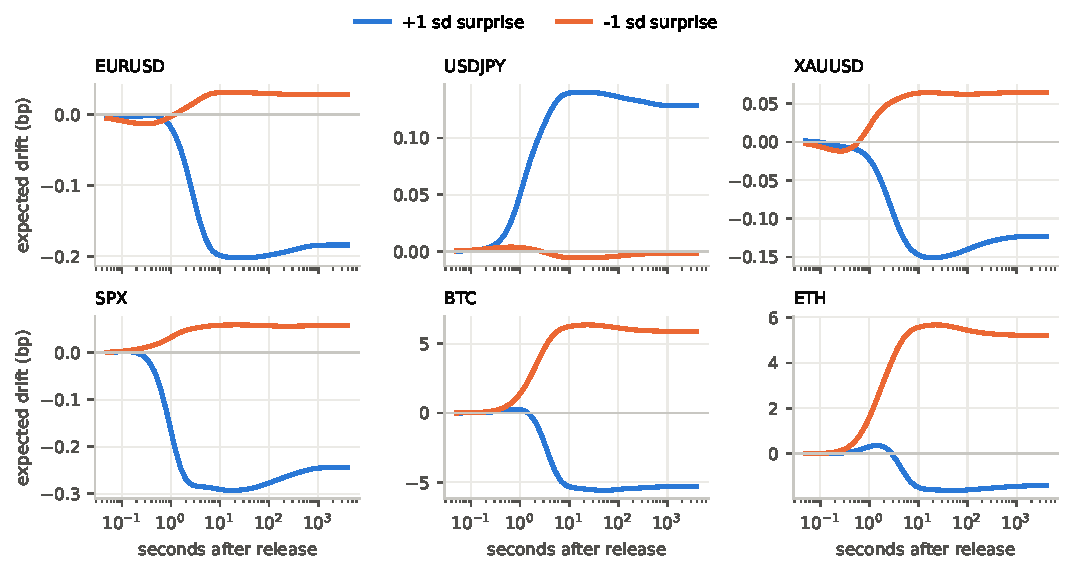
\includegraphics[width=\linewidth]{figures/drift_CPI_pooled.pdf}
\caption{Expected price-discovery curves after a $\pm1$ standard-deviation CPI surprise.}\label{fig:drift}
\end{figure}

\begin{table}[!htbp]\centering\small
\caption{Expected price drift (basis points, end of window) after a $+1$ standard-deviation
surprise. $^\ast$As in Table~\ref{tab:absorption}.}\label{tab:drift}
\setlength{\tabcolsep}{4pt}
\begin{tabular}{lcccccc}
\toprule
Release & EURUSD & USDJPY & Gold & S\&P 500 & BTC & ETH \\
\midrule
CPI & $-$0.2 & $+$0.1 & $-$0.1 & $-$0.2 & $-$5.3 & $-$1.4 \\
NFP & $-$0.1 & $+$0.1 & $+$0.1 & $+$0.2 & $-$0.3 & $-$1.5 \\
PPI & 0.0 & $+$0.1 & $-$0.2 & $-$0.3 & $-$2.4 & $-$2.1 \\
FOMC & 0.0 & $-$0.1 & $+$0.1 & $+$0.1 & $-$0.3 & $+$0.2 \\
Retail & $+$0.1 & $-$0.1 & $+$0.2 & 0.0 & $-$1.3 & $-$0.5 \\
\midrule
GDP$^\ast$ & $+$0.1 & $-$0.1 & $-$0.1 & 0.0 & $+$0.9 & $+$0.2 \\
FOMC press conf.$^\ast$ & 0.0 & 0.0 & 0.0 & $+$0.1 & 0.0 & $+$0.1 \\
Claims$^\ast$ & 0.0 & 0.0 & 0.0 & 0.0 & $+$0.4 & $+$0.6 \\
ECB$^\ast$ & 0.0 & 0.0 & 0.0 & 0.0 & $-$0.1 & $-$0.1 \\
ECB press conf.$^\ast$ & 0.0 & 0.0 & 0.0 & 0.0 & $-$0.3 & $-$0.3 \\
BoJ$^\ast$ & 0.0 & 0.0 & 0.0 & 0.0 & $-$0.1 & $+$0.3 \\
\bottomrule
\end{tabular}
\end{table}

\paragraph{Goodness of fit.} Time-rescaled residuals \citep{brown2002time} have
Kolmogorov--Smirnov statistics of at most \ksMax{} against Exp(1); the per-window
excess-dispersion test rejects in \edLo--\edHi\% of windows, compared with 42\% (power-law
kernel) and 93\% (double exponential) reported for FX data by \citet{rambaldi2015modeling}.

\paragraph{Forecasting the post-release burst.} On the \nTestReleases{} releases of 2025--2026,
an MSX model fitted on 2022--2024 forecasts the number of $\delta$-crossings in the first 1, 5
and 15 minutes in closed form (Table~\ref{tab:track-d}). It improves on same-type climatology
at every horizon but is beaten by the \bestActivityModel{} and HAR regressions, which are fitted
directly to this target; we report this negative result as is. For the direction of the move
the structural model is informative: the correlation between its forecast and the realised
one-minute drift is \driftCorrOursOne{}, against \driftCorrBaseOne{} for the best baseline.

\begin{table}[!htbp]\centering\small
\caption{Post-release activity forecasts on the \nTestReleases{} test releases (mean over
assets; lower is better). Bold: best; underlined: second best; shaded: our model.}\label{tab:track-d}
\setlength{\tabcolsep}{5pt}
\begin{tabular}{lrrrrrr}
\toprule
& \multicolumn{3}{c}{RMSE of $\log(1+N)$} & \multicolumn{3}{c}{QLIKE of realised variance} \\
\cmidrule(lr){2-4}\cmidrule(lr){5-7}
Method & 1 min & 5 min & 15 min & 1 min & 5 min & 15 min \\
\midrule
Climatology & 1.440 & 1.308 & 1.199 & \textbf{1.263} & 0.916 & 0.701 \\
Event-study OLS & \textbf{1.140} & \textbf{0.925} & \textbf{0.776} & 2.552 & \textbf{0.580} & \textbf{0.372} \\
HAR & \underline{1.217} & \underline{0.985} & \underline{0.820} & \underline{1.467} & \underline{0.762} & \underline{0.468} \\
\rowcolor{oursbg} MSX closed form & 1.322 & 1.049 & 0.955 & 2.913 & 1.036 & 0.518 \\
\bottomrule
\end{tabular}
\end{table}
